\chapter{Preliminaries}
\label{chap:preliminaries}
In this chapter we give a brief introduction to the relational-database
normalization. However, the chapter is intended to be used only as quick reference,
since discussing the relational data model and the relational-database normalization
in detail will be out of the scope of this report. For readers who would like to read
more on the subject we recommend the textbook by Elmasri and Navathe~\cite{bdb1} or
the textbook by Kemper and Eickler~\cite{bdb2} for German speaking readers, both of which have 
proven to be helpful guides throughout the development process of LDBN. There also
many free on-line resources such as the article 
\textit{A Simple Guide to Five Normal Forms in Relational Database Theory}
by Kent~\cite{p7}.  

\section{Definitions}
In the following we give some very important definitions to some key
concepts in the relational-database
normalization, such as relation, key, functional dependency, lossless-join, 
2NF, 3NF, BCNF and others. We also provide the reader with examples to illustrate the 
different normalization concepts in practice. We follow the notations 
of Kemper and Eickler~\cite{bdb2}. 
All of the following definitions excluding the examples are also taken from~\cite{bdb2},
Chapter~6.  

\subsection{Relation}
In relational databases data is represented in tables/relations. 
The columns in the table/relation identify the attributes, for instance
in a table for storing personal data for students such attributes could be
name, date of birth and so forth. A row or a tuple contains all the data of a single 
instance of the table such as a student named John Doe.
In the relational model, every row must have a unique identification or 
key based on the data. Figure~\ref{fig:rmodel} shows an example of a relation, in which 
the matriculation number is the key that uniquely identifies each row/tuple in the relation.

\begin{figure}[h]
  \begin{center}
    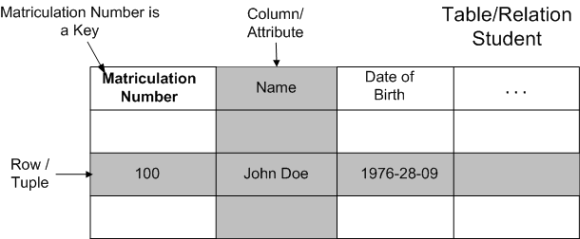
\includegraphics[width=0.85\textwidth]{./img/rmodel01.png}
    \caption{Relation Example}
    \label{fig:rmodel}
  \end{center}
\end{figure}

\subsection{Key}
As we mention a key is used to uniquely  identify a tuple. Each table can contain
more than one key. For example,
in our \textit{Student Relation} we could also have an attribute \textit{Personal Number} 
which can also be used
as a key. Furthermore, each key may be composed from more than one attribute, for instance, 
all the attributes of every relation always build a key. However, such a key can often be reduced
to a smaller subset of the relation's attributes. 
We refer to keys that cannot be reduces any more without loosing their key property as candidate keys.
In addition, each relation has a primary key, which is an instance of a candidate key for that relation.

\subsection{Functional Dependency}
The concept of Functional Dependency (FD) is central to normalization theory. 
FD is a semantic concept, which describes particular semantic relationship 
between the attributes of a relationship. A FD is often represented as $\alpha$ $\rightarrow$ $\beta$, 
where $\alpha$ and $\beta$ are subsets of the attributes of a given relation \textit{R}.
We often refer to $\alpha$ as the left-hand side (LHS) of the FD and to $\beta$ as the 
right-hand side (RHS) of the FD.
Furthermore, the representation $\alpha$ $\rightarrow$ $\beta$ means that $\beta$ is 
functionally dependent on $\alpha$ if and only if 
for each value of $\alpha$ no more than one value of $\beta$ is associated. 
More formally, if \textit{t} and \textit{r} are two tuples in the relation \textit{R}
with \textit{t.a = r.a} then \textit{t.b = r.b}. Here
\textit{t.a = r.a} is a short form for 
\begin{math} \forall A \in \alpha : t.A= r.A \end{math}.  
In other words, the values of the attributes  in $\alpha$ uniquely 
determines the values of of the attributes in $\beta$ and 
if there were several tuples that had the same value of $\alpha$ then all these 
tuples will have an identical values for the attributes in $\beta$. 

We would like to illustrate this very important concept of FDs with an example. 
Let us consider the following relation $R = \{A, B, C, D\}$. 
The The example comes from~\cite{bdb2}, Section 6.1.

\begin{center}
\begin{tabular}[h]{l|l|l|l|l|}
  \cline{2-5}
  & \multicolumn{4}{|c|}{$R$} \\ \cline{2-5}
  & $A$ & $B$ & $C$ & $D$ \\ \cline{2-5}
  $t$ & $a_4$ & $b_2$ & $c_4$ & $d_3$ \\ 
  $p$ & $a_1$ & $b_1$ & $c_1$ & $d_1$ \\ 
  $q$ & $a_1$ & $b_1$ & $c_1$ & $d_2$ \\ 
  $r$ & $a_2$ & $b_2$ & $c_3$ & $d_2$ \\ 
  $s$ & $a_3$ & $b_2$ & $c_4$ & $d_3$ \\ \cline{2-5}
\end{tabular}
\end{center}

It can be stated that $A \rightarrow B$  is satisfied, thus
$B$ is functionally dependent on $A$ or \textit{A determines B}.
As all $A$ tuples that have the same value have the same $B$ value. However,
$B \rightarrow A$ is \textbf{not} satisfied, since the tuples $r$ and $s$ with $r.B = s.B$ have
different $A$ values. Other FDs in the relation which are also satisfied are
$A \rightarrow C$ and $C, D \rightarrow B$.

Functional dependency is \textit{trivial} if it satisfied by all tuples, i.e., $\alpha$ $\rightarrow$ $\alpha$.
In general, a functional dependency of the form $\alpha$ $\rightarrow$ $\beta$ is trivial if 
$\beta \subseteq \alpha$.

\subsection{Closure of a Set of FDs}
In a relationship $R$ with a set of FDs $F$ we define the closure of $F$ or simply $F+$
as a set of all possible FDs which can be derived from the original set of FDs $F$. In 
other words, $F+$ is the set of all FDs that must always hold in $R$. $F+$ can be
logically implied using inference rules called \textit{Armstrong's Axioms}. 
Repeated application of these rules will generate all functional dependencies in the closure F+.

Let $\alpha, \beta, \gamma$ and $\delta$ are subsets of the Attributes in $R$, then:

\begin{description}
  \item[Reflexivity Rule] If $\beta \subseteq \alpha$ then $\alpha \rightarrow \beta$.
  \item[Augmentation Rule] If $\alpha \rightarrow \beta$ then $\alpha\gamma \rightarrow \beta\gamma$, where $\alpha\gamma$ is a short form of $\alpha \cup \gamma$.
  \item[Transitivity Rule] If $\alpha \rightarrow \beta$ and $\beta \rightarrow \gamma$ then $\alpha \rightarrow \gamma$.
\end{description}

\noindent Additional rules which can be derived from above axioms:

\begin{description}
  \item[Union Rule] If $\alpha \rightarrow \beta$ and $\alpha \rightarrow \gamma$ then $\alpha \rightarrow \beta\gamma$.
  \item[Decomposition Rule] If $\alpha \rightarrow \beta\gamma$ then $\alpha \rightarrow \beta$ and $\alpha \rightarrow \gamma$.
  \item[Pseudo Transitivity Rule] If $\alpha \rightarrow \beta$ and $\gamma\beta \rightarrow \delta$ then $\alpha\gamma \rightarrow \delta$.
\end{description}

Here follows a short example on how to apply the different rules. 
Let us consider the following relation:\\ \\
\indent $R = \{A, B, C, G, H, I\}$ \\
\indent $F = \{A \rightarrow B, A \rightarrow C, B \rightarrow H, CG \rightarrow H, CG \rightarrow I\} $ \\

Among others the following FDs can be inferred:\\
\indent \begin{tabular}[h]{r l}
  $A \rightarrow H$ & by applying the Transitivity Rule: $A \rightarrow B, B \rightarrow H$ \\
  $CG \rightarrow HI$ & by  applying the Union Rule: $CG \rightarrow H, CG \rightarrow I$ \\
  $AG \rightarrow I$ & by first applying the Augmentation Rule: $A \rightarrow C, AG \rightarrow CG$; \\
  $ $ & and then applying the Transitivity Rule: $AG \rightarrow CG, CG \rightarrow I$
\end{tabular}

\subsection{Formal Definition of Keys}
With the help of FDs we can now define keys of a relation more formally. 
But first we define 
the concept of \textbf{full functional dependence}. 
Let $\alpha$ and $\beta$ be sets of attributes.
$\beta$ is \textbf{fully functionally dependent} on $\alpha$ if both of the following criteria are true:
\begin{enumerate}
  \item $\alpha \rightarrow \beta$
  \item $\alpha$ cannot be reduced, i.e., $\forall A \in \alpha : \alpha - \{A\} \nrightarrow \beta$ 
\end{enumerate}
 
Let $R$ be a relation with $\alpha \subseteq R$, then $\alpha$ is a \textbf{superkey} if $\alpha \rightarrow R$. 
$\alpha$ is called \textbf{candidate key} if $R$ is fully functional dependent on $\alpha$. 
There can be many candidate keys in a relation. Each relation has one \textbf{primary key},
which is a instance of a candidate key. Furthermore, we define an attribute as \textbf{prime} or
\textbf{key attribute} if 
it is part of any candidate key in $R$. 



\subsection{Cover of Sets of FDs}
Equivalent sets of functional dependencies are called covers of each other.
There are many different equivalent sets of FDs. 

Two sets of FDs $F$ and $G$ are equivalent ($F \equiv G$)
if and only if their closures are equal, i.e., $F+ = G+$. This means for a given set of FDs $F$ there is 
only one unique closure $F+$~\cite{bdb2}. Furthermore every set of functional dependencies 
has a minimal/canonical cover - $F_c$. Unlike the closure $F+$ the minimal cover $F_c$ is not unique. 
Every cover which satisfies the following properties is called minimal/canonical cover of $F$:

\begin{enumerate}
  \item $F_c \equiv F$, i.e., $F_{c}+ = F+$
  \item We cannot delete any attribute from any FD and have an equivalent set of FDs.
  \item Every left-hand side of each FD must be unique. This can be done by successively applying the \textit{Union Rule}.
\end{enumerate}

An example: for the relational scheme $R = \{A, B, C\}$, and the set $F$ of functional dependencies: \\

$ F = \{A \rightarrow BC, B \rightarrow C, A \rightarrow B, AB \rightarrow C\}$ \\
\indent The set $F_c = \{A \rightarrow B, B \rightarrow C\}$ is a canonical cover of $F$. \\
\indent Proof:
\indent \begin{enumerate}
  \item $F \equiv F_c $, by applying the \textit{Armstrong's Axioms} it can be shown that $A \rightarrow BC$ and $AB \rightarrow C$ are in $F_{c} + $, thus the two sets are equivalent.
  \item We cannot remove any attributes from the two FDs in $F_c$, because by doing so they will become trivial and the resulted set will not be equivalent to $F_c$.
  \item Both of the FDs in $F_c$ have a unique LHS. 
\end{enumerate}


\subsection{Decomposition of Relations}
\label{sec:decofrel}
Relational-database normalization typically involves decomposing a relation $R$
into two or more relations $R_1,...,R_n$, with $R_i \subseteq R$, i.e., the 
new relations contain a subset of the original attributes. 
In order for the decomposition to yield
exactly the same information as the original relation the new relations have to be
combined (joined). However, they are two major criteria that have to be considered when
decomposing a relation:

\begin{enumerate}
  \item \textit{Lossless Join Property:} ensures that no information is lost during the decomposition process.
  \item \textit{Dependency Preservation Property:} ensures that all the FDs from the original relation hold in the new set of relations. 
\end{enumerate}

\subsubsection{Lossless Join}
The decomposition of $R$ into $R_1,...,R_n$ has a \textit{lossless-join} if for
any instance $r$ of $R$ that satisfies the condition: $$r = r_1 \Join ... \Join r_n \mbox{, with } r_i \mbox{ is the short form of } \Pi_{R_{i}} (r) \mbox{ for } 1 \leq i \leq n$$ 
Thus the information contained in $r$ must be reconstructible by using the natural join~($\Join$) on the relations $R_1,...,R_n$. 

We can also define criteria for \textit{lossless join} by using FDs. 
A decomposition of $R$ into $R_1$ and $R_2$ has \textit{lossless-join} 
if at least one of the following FDs are in $F+$:
\begin{enumerate}
  \item $R_1 \cap R_2 \rightarrow R_1 $ 
  \item $R_1 \cap R_2 \rightarrow R_2 $
\end{enumerate}

The above conditions ensure that the attributes involved in the natural join 
($R_1 \cap R_2$) build a candidate key for at least one of the two relations. This ensures that 
we can never get the situation where spurious tuples are generated, as for any 
value on the join attributes there will be a unique tuple in one of the relations. 

Figure~\ref{fig:lossy} is illustrating a decomposition of a relation $R = \{A, B, C \}$ with
a set of FDs $F = \{B \rightarrow C, C \rightarrow B\}$. As can be seen, the decomposition is 
not satisfying the lossless join property. We can also prove this by showing that the FDs: 
$A \rightarrow AC \notin F+$ and $A \rightarrow AB \notin F+$.
It should be mentioned that in relational-database normalization additional or spurious tuples, which were
not present in the original relation but can be found in the joined relation, are also considered as information loss. 
Figure~\ref{fig:lossless} shows
a lossless-join decomposition of the same relation. Here the requirement for lossless join is satisfied,
since $C \rightarrow BC \in F+$.

\begin{figure}[h]
  \centering
  \subfigure[Lossy]{
    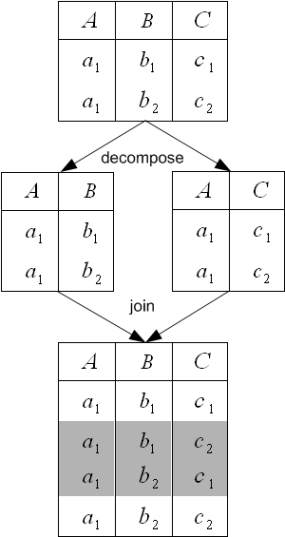
\includegraphics[scale=0.5]{./img/lossy01.png}
    \label{fig:lossy}
  }
  \subfigure[Lossless]{
    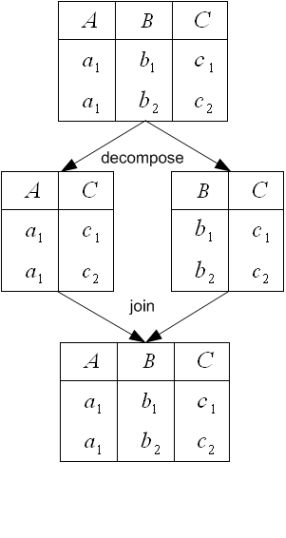
\includegraphics[scale=0.5]{./img/lossless01.png}
    \label{fig:lossless}
  }
\caption{Lossless Join Property Example}
\end{figure}

\subsubsection{Dependency Preservation}
Another desirable property in database design is dependency preservation. 
Let $F$ be a set FDs that hold in $R$, which is decomposed in relations $R_1 ,..., R_n$.
We can partition the dependencies given by $F$ such that $F_1 ,..., F_n$
are dependencies that only involve attributes from relations $R_1 ,..., R_n$ respectively. 
If the following condition is satisfied then we say that the decomposition is 
dependency preserving, otherwise it is not: 
\begin{displaymath}
F \equiv (F_1 \cup ... \cup F_n ) \mbox{  respectively  } F+ = (F_1 \cup ... \cup F_n ) +
\end{displaymath}

In the following we illustrate the concept of dependency preservation with an example
of a decomposition which is not satisfying this property: \\ \\
\indent $R = \{A, B, C, D\}$ \\
\indent $F = \{ABC \rightarrow D, D \rightarrow AB\}$ \\
\indent Decompose $R$ in: \\
\indent \begin{tabular}[h]{l l}
  $R_1 = \{C, D\}$  & $F_1 = \{ \}$ \\
  $R_2 = \{A,B,D\}$ & $F_2 = \{D \rightarrow AB \}$ \\
\end{tabular} \\

The decomposition is lossless-join, since $D \rightarrow ABD \in F+$. However, 
the decomposition is \textbf{not} dependency preserving, because the FD $ABC \rightarrow D \in F+$ but it is
not present in $(F_1 \cup F_2) +$.

\section{Brief Introduction to the Normal Forms}
\label{sec:nfintro}
In the previous section we discussed some aspects on how to decompose a relation correctly, 
in this section we will continue this discussion by introducing some of the normal forms
namely the Fist Normal Form (1NF), Second Normal Form (2NF), Third Normal Form (3NF) and
Boyce-Codd Normal Form (BCNF). Normal forms are formal
notations, which are used to avoid or eliminate the three types of data anomalies 
(insertion, deletion and update anomalies) which a database may suffer from. 
These concepts are clarified in the next section, after that we
define the different normal forms.

\subsection{Data Anomalies}
A relation that is not sufficiently normalized can suffer from logical inconsistencies of various types
called data anomalies. We illustrate the the different data anomalies by
giving an example of a relation which suffers from all three anomalies: Insertion, Update and
Delete Anomaly. The following table
shows the relation \textit{Student Courses}, which stores data about a student and the courses 
that he/she has taken. In addition, each student is assigned to a mentor, who is 
a professor from the student's department. 

\bgroup
\setlength\LTleft{-2cm}\setlength\LTright{-2cm}%
\LTXtable{\textwidth}{./tex/relation-sc.tex}
\egroup

\begin{description}
  \item[Insertion Anomaly] means that that some data can not be 
    inserted in the database. For example we can not add a new course to the \textit{Student Courses}
    relation, unless we insert a student who has taken that course.
  \item[Update Anomaly] means we have data redundancy in the database and to make any 
    modification we have to change all copies of the redundant data or else the 
    database will contain incorrect data. For example in our database we have the course 
    \textit{Database Concepts} which appears in several tuples in our relation. 
    To change its description to \textit{New Database Concepts} we have to change 
    it in all tuples. Indeed one of the purposes of normalization is to eliminate data 
    redundancy in the database.
  \item[Deletion Anomaly] means deleting some data cause other information to be lost. 
    For example if student Eriksson is deleted from the relation we also lose the 
    information that we had a course \textit{Distributed Systems}.
\end{description}

\subsection{First Normal Form} 
A relation is in first normal form (1NF) if all its attributes are simple or atomic. 
In other words, none of the attributes of the relation is a compositition of multiple attributes, 
a set of values nor a relation. The following relation is not in 1NF:

\begin{center}
\begin{tabular}[h]{|l|l|l|l|}
  \hline
  Matrl.Nr. & Surname & Data-of-Birth & Taken-Courses \\ \hline
  100 & John & 1976-09-28 & \{Database Concepts, Operating Systems \} \\  
  200 & Schmidt & 1986-05-19 & \{Database Concepts, Operating Systems,  \\ 
      &         &            & Computer Networks \} \\
  300 & Eriksson & 1984-02-29 & \{Distributed Systems \} \\ \hline
\end{tabular}
\end{center}

The attribute \textit{Taken-Courses} is violating the 1NF rule, since it is a set of 
course names. To avoid this we can use a relation similar to the \textit{Student Courses} relation,
which is in 1NF. However, it was shown in the previous section that the relation suffers
from all three data anomalies, therefore we need further restrictions to the 1NF. We
introduce these in the following sections.  

\subsection{Second Normal From}
A relation is in 2NF if it is in 1NF and all its non-key attributes are fully
functionally dependent on every candidate key of the relation.
Note that key attributes are those attributes, which are parts of any 
candidate key, and non-key attributes do not participate in any candidate key. 

The relation \textit{Student Courses} is not in 2NF. In order to prove this we must
fist define a set of FDs for the relation. Figure~\ref{fig:fds01a} is a graphical representation 
of the functional dependencies between the primary key \textit{Matrl.Nr., Course ID} and the rest of the 
attributes of the \textit{Student Courses} relation. 
Note that the attribute to the right of the arrow is functionally dependent on the attribute 
in the left of the arrow.  

\begin{figure}[h]
  \begin{center}
    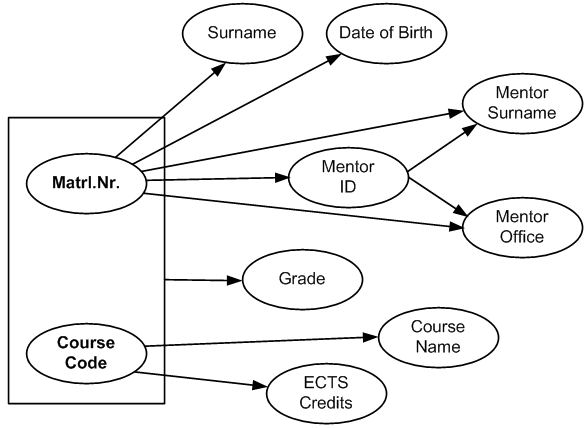
\includegraphics[width=0.6\textwidth]{./img/fds01a.png}
    \caption{Set of FDs which hold in \textit{Student Courses}}
    \label{fig:fds01a}
  \end{center}
\end{figure}

As can be seen only the \textit{Grade} attribute is fully functionally dependent on the primary key.
On the other hand, the attributes \textit{Surname, Date of Birth, Mentor ID, Mentor Surname, Course Name, ECTS Credits} 
and \textit{Grade} are all non-key attributes because non of them is a component of a candidate key, therefore
the relation is not in 2NF. 

To convert \textit{Student Courses} to 2NF we have to make all non-primary attributes 
to be fully functionally dependent on the primary key. 
To do that we need to decompose the \textit{Student Courses} relation into the following three new relations:
\textit{Student = \{Matrl.Nr., Surname,  Date of Birth, Mentor ID, Mentor Surname\}}, 
\textit{Courses = \{Course ID, Course Name, ECTS Credits\}} and 
\textit{Grades = \{Matrl.Nr., Course ID,  Grade\}}.
Following are these three relations and their contents:

\begin{center}
\begin{tabular}[h]{|c|c|c|c|c|c|}
\hline
\multicolumn{6}{|c|}{\textit{Students and Mentors}} \\ \hline
\textbf{Matrl.Nr.} & Surname & Date of & Mentor & Mentor  & Mentor \\
                   &         & Birth   & ID     & Surname & Office \\
 \hline \hline
 100 & John     & 1976-09-28 & 101 & Codd   & B707 \\
 200 & Schmidt  & 1986-05-19 & 201 & Turing & A612 \\
 300 & Eriksson & 1984-02-29 & 101 & Codd   & B707 \\ \hline
\end{tabular} 
\end{center}

\begin{center}
\begin{tabular}[h]{|c|c|c|}
\hline
\multicolumn{3}{|c|}{\textit{Courses}} \\ \hline
\textbf{Course Code} & Course Name & ECTS Credits \\
\hline \hline
5DV001 & Database Concepts   & 7.5 \\ 
5DV002 & Operating  Systems  & 7.5 \\
5DV003 & Computer  Networks  & 7.5 \\
5DV004 & Distributed Systems & 7.5 \\ \hline
\end{tabular}
\end{center}

\begin{center}
\begin{tabular}[h]{|c|c|c|}
  \hline
  \multicolumn{3}{|c|}{\textit{Grades}} \\ \hline
  \textbf{Matrl.Nr.} & \textbf{Course Code} & Grade \\
  \hline \hline
  100 & 1 & A \\ 
  100 & 2 & B \\
  200 & 1 & B \\
  200 & 2 & B \\
  200 & 3 & C \\
  300 & 4 & A \\ \hline
\end{tabular}
\end{center}

All three relations are in 2NF. Furthermore, it can be proven that the
decomposition is lossless and dependency preserving. 
Examination of the new relations shows that we have eliminated most of the redundancy 
in the database. The relations \textit{Courses} and \textit{Grades} are free
from any data anomalies. However, the \textit{Students~and Mentors} relation still suffers form all three
data anomalies, because it also keeps track of all mentors:
\begin{enumerate}
  \item We cannot add new mentors without adding new students.
  \item To change the office of a mentor we have to update several tuples.
  \item If the student Schmidt is deleted we also lose the information about the mentor Turing.
\end{enumerate}
 
\subsection{Third Normal Form}
A relation $R$ is in 3NF if it is in 2NF and for all FDs that hold in $R$
of the form $\alpha \rightarrow B$, where $\alpha \subseteq  R$ and $B \in R$, 
at least one of the following holds: 
\begin{enumerate}
  \item $B \in \alpha$, i.e., the FD is trivial
  \item $B$ is a prime attribute, i.e., $B$ is part of a candidate key.
  \item $\alpha$ is a superkey of $R$.
\end{enumerate}

From the three previous relations only the \textit{Students and Mentors} one is not in 3NF, since 
the FD \textit{Mentor~ID $\rightarrow$ Mentor~Surname, Mentor~Office} holds in the relation but 
it violates the 3NF property. Therefore we need to further decompose the relation into two
new relation: \textit{Students~= \{Matrl.Nr., Surname,Data~of~Birth, Mentor~ID\}} and
\textit{Mentors~= \{Mentor~ID, Mentor Surname, Mentor Office\}}. The following two tables represent
the two new relations and their content.

\begin{table}[ht]
\begin{minipage}[t]{0.5\linewidth}\centering
\begin{tabular}{|c|c|c|c|}
\hline
\multicolumn{4}{|c|}{\textit{Students}} \\
\hline
\textbf{Matrl.Nr.} & Surname & Date of  & Mentor \\
                   &         & Birth    & ID     \\
\hline \hline
100 & John     & 1976-09-28 & 101 \\
200 & Schmidt  & 1986-05-19 & 202 \\
300 & Eriksson & 1984-02-29 & 101 \\
\hline
\end{tabular}
\end{minipage}
\hspace{0.5cm}
\begin{minipage}[t]{0.5\linewidth}
\centering
\begin{tabular}{|c|c|c|}
\hline
\multicolumn{3}{|c|}{\textit{Mentors}} \\ \hline
 \textbf{Mentor} & Mentor  & Mentor \\
 \textbf{ID}     & Surname & Office \\
 \hline \hline
 101 & Codd   & B707 \\
 201 & Turing & A612 \\ \hline
\end{tabular}
\end{minipage}
\end{table}

It can be shown that the two new relation are in 3NF. Furthermore, the 
decomposition is lossless-join and dependency-preserving. Indeed it is always 
possible to find a dependency-preserving lossless-join decomposition which is in 3NF~\cite{bdb2}, Section~6.8.
However, a 3NF decomposition does not necessarily satisfy these properties. Consider the following example
of a 3NF decomposition which is not dependency preserving:

\begin{center}
\begin{tabular}[h]{l l}
  $R = \{A, B, C, D\}$ & $F = \{A \rightarrow BC, C \rightarrow D, D \rightarrow B\}$ \\
  Decompose $R$ in:  & $R_1 = \{A, B, C\} \mbox{ and } R_2 = \{C,D\}$ \\ 
\end{tabular}
\end{center}

It is worth noting that our original relation \textit{Student Courses} is now decomposed
into four different relations: \textit{Students, Mentors, Courses} and \textit{Grades}. The 
decomposition is in 3NF, this means that each member of the set of relation schemes is in 3NF. 
More importantly, the decomposition does not suffer from free from any data anomalies. 
Let us clarify this in more detail:
\begin{description}
  \item[Insertion Anomaly:] Now new mentors and courses can be inserted to the relation mentors/courses without needing to add new students.
  \item[Update anomaly:] Since redundancy of the data was eliminated no update anomaly can occur. For example, to change the \textit{Course Name} for 5DV001 only one change is needed in the relation \textit{Courses}.
  \item[Deletion anomaly:]  The deletion of student Schmidt from the database is achieved by deleting Schmidt's records from both \textit{Students} and \textit{Grades} relations and this does not have any side effects on the different courses or mentors, since they stay untouched in their own relations.  
\end{description}

\subsection{Boyce-Codd Normal Form}
\label{sec:BCNF}
BCNF is a slightly stronger version of 3NF. A relation scheme $R$ is in BCNF 
with respect to a set $F$ of FDs if $R$ is in 3NF and for all functional dependencies in $F+$ 
of the form $\alpha \rightarrow \beta$, where $\alpha \subseteq R$ and $\beta \subseteq R$,
at least one of the following holds:
\begin{enumerate}
  \item $\alpha \rightarrow \beta$ is a trivial functional dependency (i.e. $\beta \subseteq \alpha$)
  \item $\alpha$ is a superkey for $R$ 
\end{enumerate}

Only in rare cases a 3NF relation does not meet the requirements of BCNF. Our decomposition 
\textit{\{Students, Mentors, Courses, Grades\}} is in BCNF. Let us consider the following
example of the relation {} which is in 3NF but not in BCNF.  The example 
comes from~\cite{bdb2}, Section~6.5.3.

\begin{center}
\begin{tabular}[h]{l l}
  $PostalCodeIndex = \{Street, City, Province, PostalCode\}$ & \\ [0.5ex]
  $F = \{Street, City, Province \rightarrow PostalCode; \mbox{ } PostalCode \rightarrow City, Province\}$ \\ [1.5ex]
  The FD $PostalCode \rightarrow City, Province$ is not trivial and it is not a superkey, \\ [0.5ex]
  thus the $PostalCodeIndex$ relation is not in BCNF. & \\ [1.5ex]
  BCNF decomposition of $PostalCodeIndex$:   &  \\ [0.5ex]
  $Streets =\{PostalCode, Street\}$ & \\ [0.5ex]
  $Cities = \{PostalCode, City, Province\}$ & \\ [0.5ex]
\end{tabular}
\end{center}

The decomposition \textit{\{Streets, Cities\}} is lossless-join, but it is not dependency-preserving. 
Indeed it is not always possible to find a dependency preserving BCNF decomposition of a relation~\cite{bdb2}, Section~6.9.

